\section{Proof of Concepts}

One main part of the investigation into the CERN-Solid collaboration is the development of a \gls{poc}. The \\gls{poc} as previously agreed upon contains the creation of two independent software modules. These software modules should show how the Solid principles -- decentralizing the Web by splitting authentication, data, and application logic -- can be included into an existing Web application.

The goal of these modules is the symbiosis of decentralized stored data in a highly functional system without comprising its performance, security, or usability.

\subsection{POC 1: Commenting Module for Events in Indico}\mbox{}\\

For the first \gls{poc} some sort of Solid-based content was planned to be enriched into the Indico system. With the product owner and chief developer of Indico, the CERN-Solid project manager and a Solid developer it was decided a commenting module for Indico events is an adequate solution to include data from an external storage entity namely a Solid pod. The ability to allow users of Indico to leave a comment on an event, which then lives in a Solid pod completely controlled by the author of the comment was concluded to be an attractive feature for Indico.

\subsubsection{Design}\mbox{}\\

For the implementation of this module several design decisions had to be made. From the fundamental choice of the module running on the client device or be computed on the server and then propagated to the client afterwards.
Other design challenges were around how to protect the resources holding the comment information. These reside on the external Solid pod and need to be fetched from the application and read by other agents. Can \glspl{acl} be configured to allow the specific use-case?

\paragraph{Client- versus Server-Side versus Microservice}\mbox{}\\

When an agent browses to a running instance of Indico most of functionality is being prepared on the server hosting Indico. It retrieves the specific request, builds the \gls{html}, and sends it to the user. For Indico most of the functionality is built with Python and the web framework Flask. Sometimes functionality needs to be closer to the user, an example is dynamic rendering of \gls{dom} elements. This is useful when new data needs to be shown right away without getting the blank white screen on page reloads.
Indico does send JavaScript, which is used client-side features, but it focuses on keeping most its features on the server.

To make the right decision if the module should be primarily developed for the client- or server-side a list of requirements to the module had to be defined. With the defined requirements in place it had to be figured out how much functionality can be extracted from existing libraries and how much needed to be implemented with the new module. Implementing existing functionality for a new programming language would defeat the \gls{poc}’s purpose of showing how an existing software could work with the Solid principles.

\begin{enumerate}
    \item Authentication with a Solid \gls{idp}
    \item (Authenticated) Requests to a Solid pod
    \item Parsing of structured data (Linked Data)
\end{enumerate}

Authentication in the Solid Ecosystem uses \gls{solidoidc}, which is an extension of the existing \gls{oidc} standard. An existing \gls{oidc} library for Python exist, but it is missing a crucial feature from the \gls{solidoidc} specification called \gls{dpop}-bound Access Tokens.

\begin{figure}
    \centering
    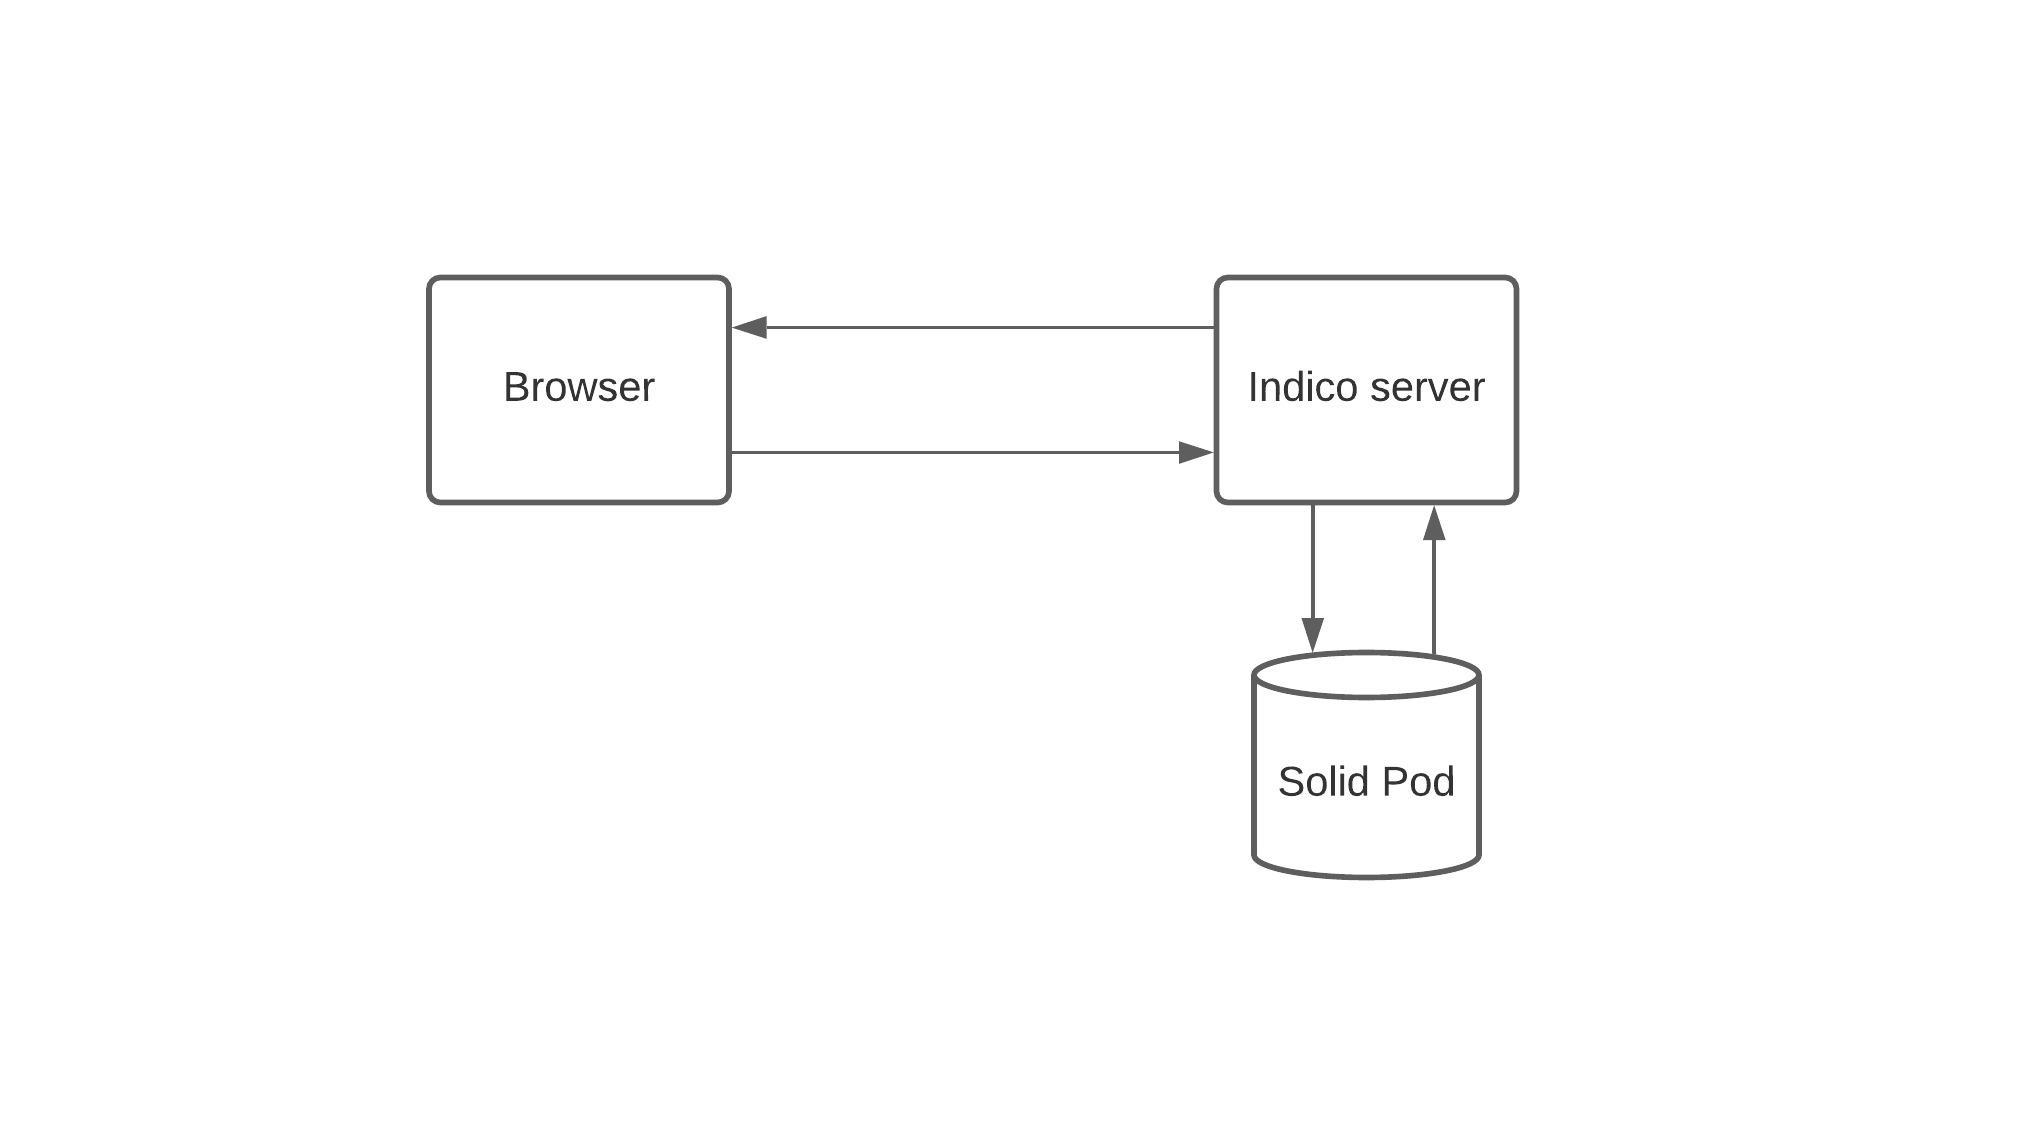
\includegraphics[width=0.8\textwidth]{prototype/graphs/poc-infrastructure-backend.jpeg}
    \caption{poc-infrastructure-backend}
    \label{fig:poc-infrastructure-backend}
\end{figure}

\begin{figure}
    \centering
    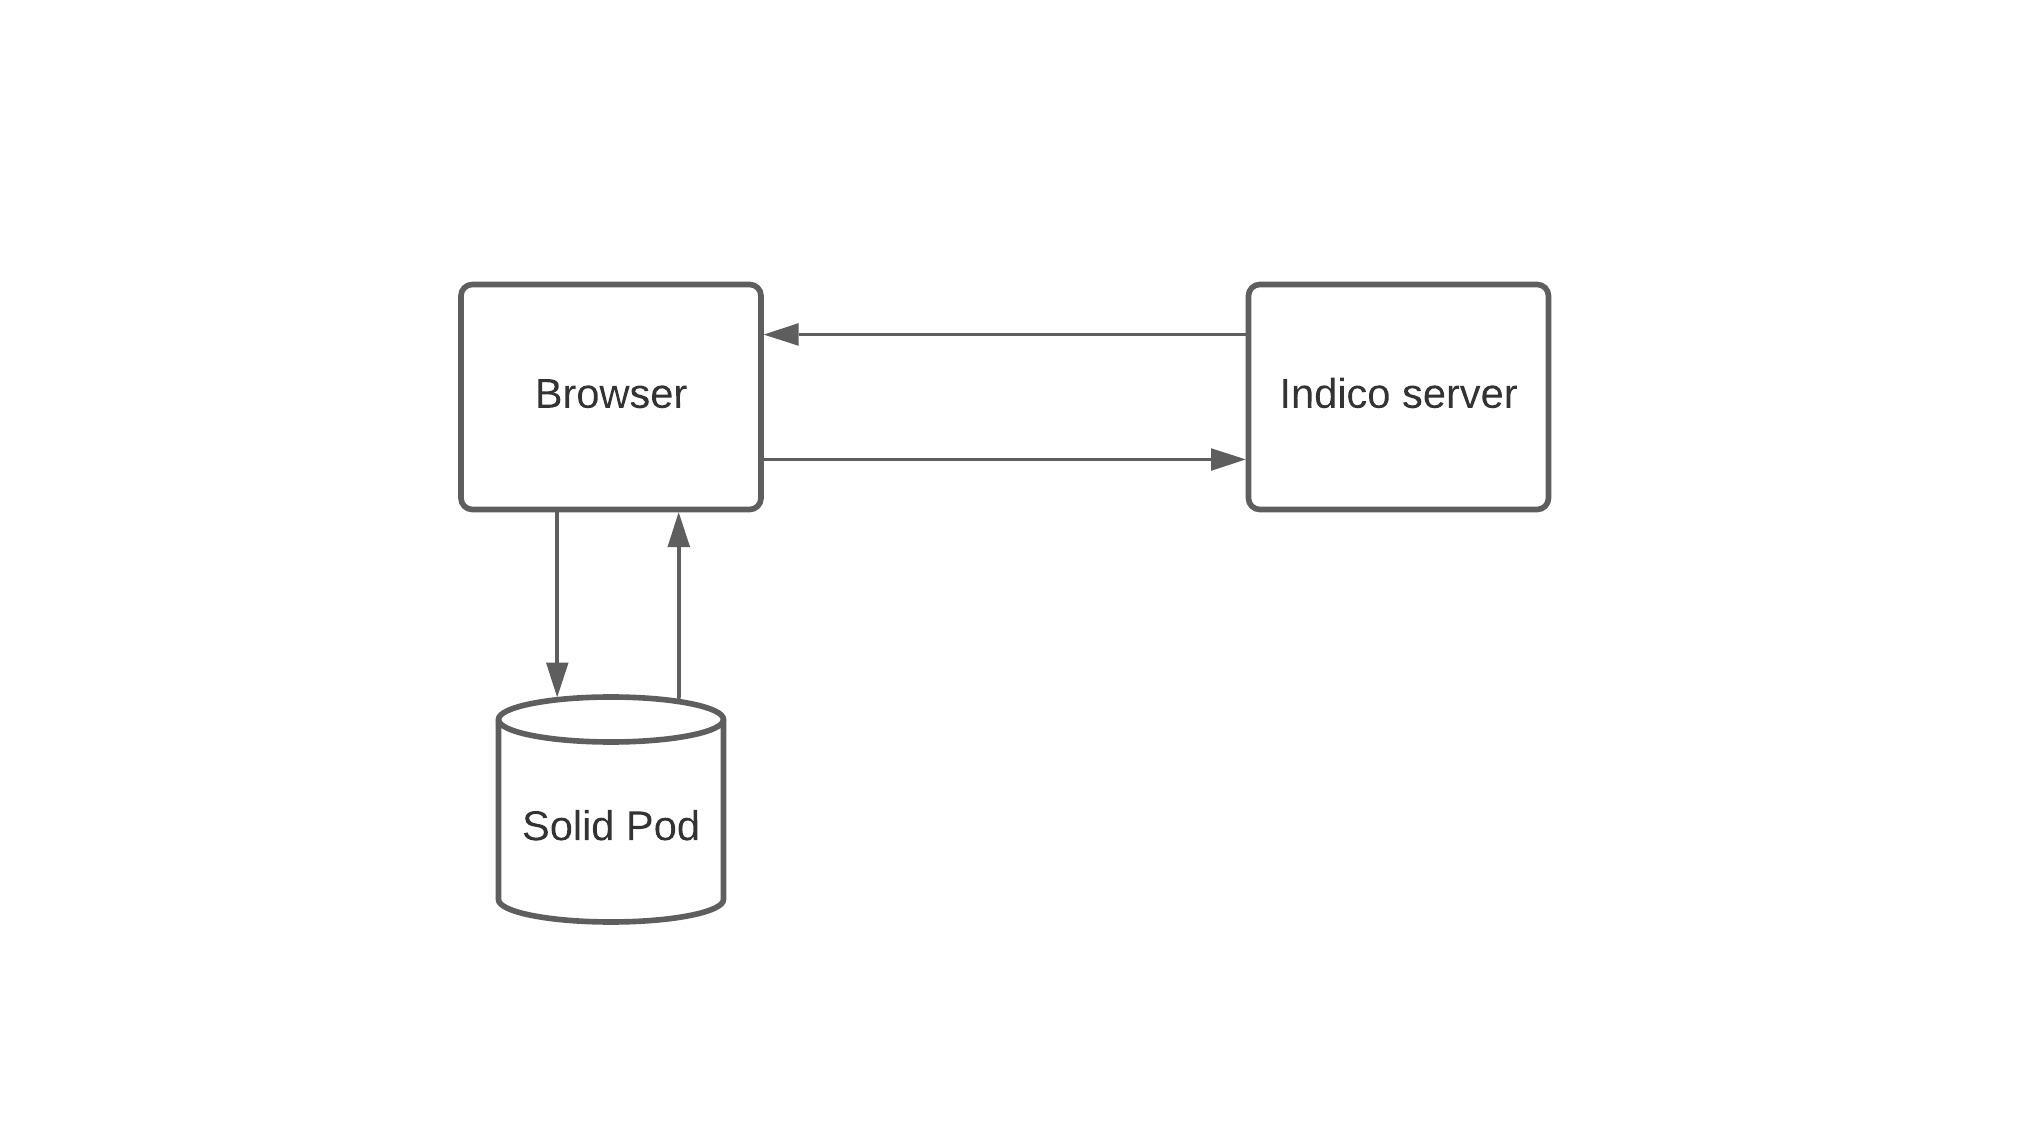
\includegraphics[width=0.8\textwidth]{prototype/graphs/poc-infrastructure-frontend.jpeg}
    \caption{poc-infrastructure-frontend}
    \label{fig:poc-infrastructure-frontend}
\end{figure}

\begin{figure}
    \centering
    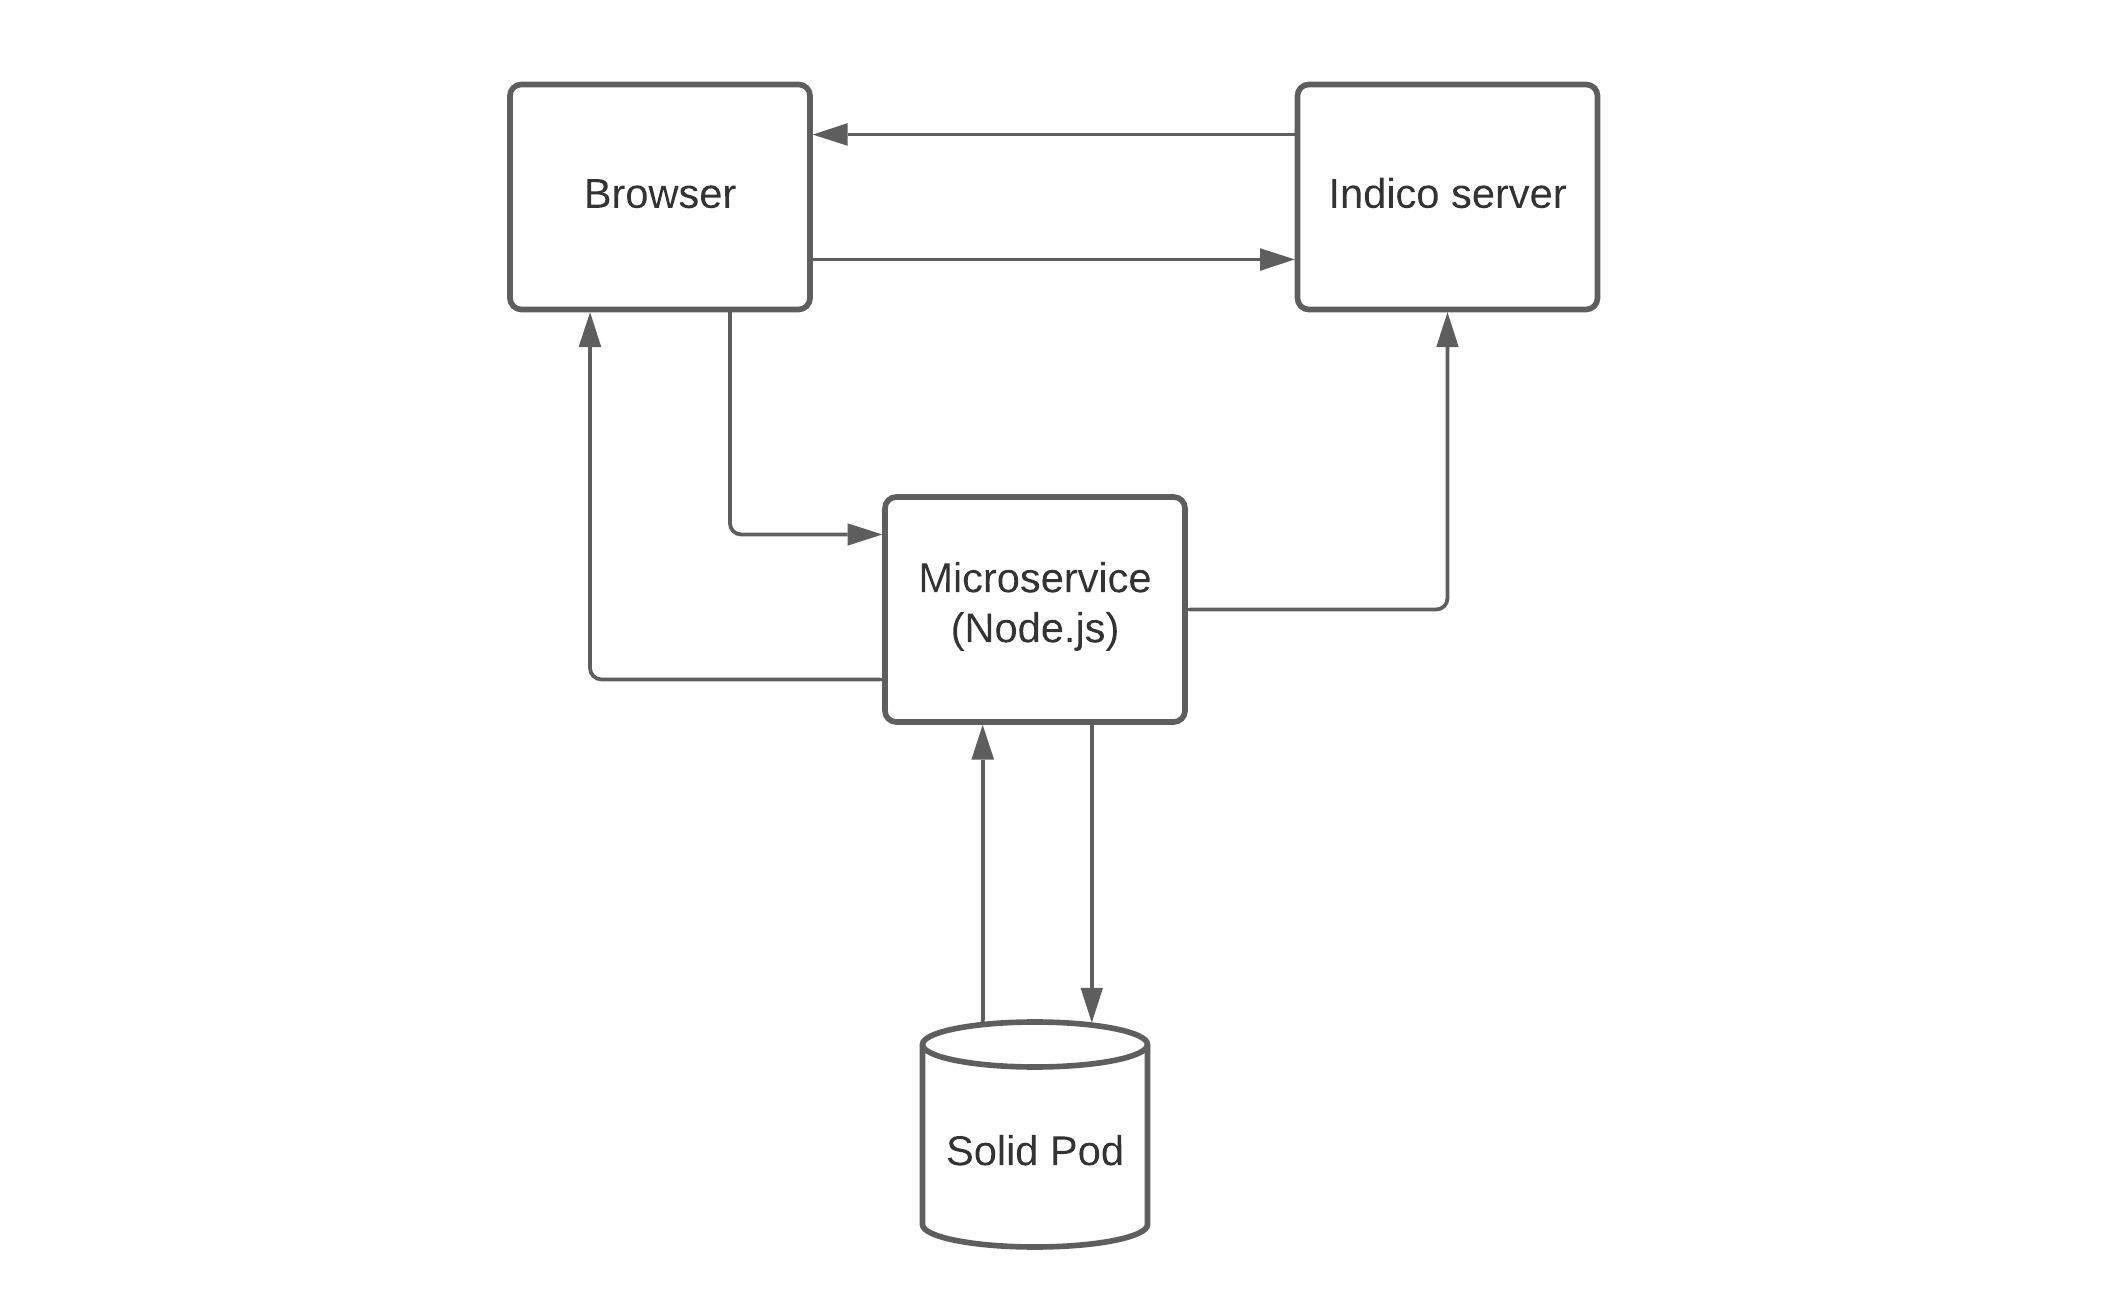
\includegraphics[width=0.8\textwidth]{prototype/graphs/poc-infrastructure-microservice.jpeg}
    \caption{poc-infrastructure-microservice}
    \label{fig:poc-infrastructure-microservice}
\end{figure}


\paragraph{Protection on Resource}\mbox{}\\

\paragraph{Modification of Resource from Pod}\mbox{}\\

\paragraph{Mitigation of Spam}\mbox{}\\

\paragraph{Giving Application Full Control of Pod}\mbox{}\\

\subsubsection{Evaluation}

\paragraph{System Description}
\paragraph{Context Diagram}
\paragraph{Stakeholders}
\paragraph{Drivers}
\paragraph{Metrics}
\paragraph{Levels}
\paragraph{Components}

\subsubsection{Analysis}

\subsection{POC 2: Auto-Complete for Conference Registration in Indico}

\subsubsection{Design}

TODO:
1st iteration, save data in pod
2nd iteration, only pull data from pod



\subsubsection{Evaluation}
\subsubsection{Analysis}

\subsection{Integration with Indico}

\subsection{Deployment of Indico Instance}
